\section{Architektura horyzontalna}

Coraz częściej aplikacje są sprzedawane jako serwisy dostępne w chmurze \cite{horizontalArchitecture}.
Pozwala to na skalowanie rozwiązań w zależności od zapotrzebowania.
Proste aplikacje pisze się w architekturze wertykalnej, co oznacza, że istnieje jedna instancja aplikacji, która wykonuje wymagane operacje.
W przypadku wzrostu zapotrzebowania na moc obliczeniową, można zaopatrzyć się w maszynę spełniającą oczekiwane wymagania.
Schemat architektury wertykalnej został zaprezentowany na rysunku \ref{rys:veriticalArchitecture}.
Takie rozwiązanie jest mało elastyczne na wahania potrzebnej mocy obliczeniowej.
Podmiana instancji wymaga zatrzymania chociaż na chwilę działania usługi.
Utrzymywanie urządzenia o dużej mocy obliczeniowej, tylko po to wytrzymało potencjalne skoki zapotrzebowania na moc obliczeniową wiąże się ze zwiększonymi kosztami.

\begin{figure}[!hb]
	\centering 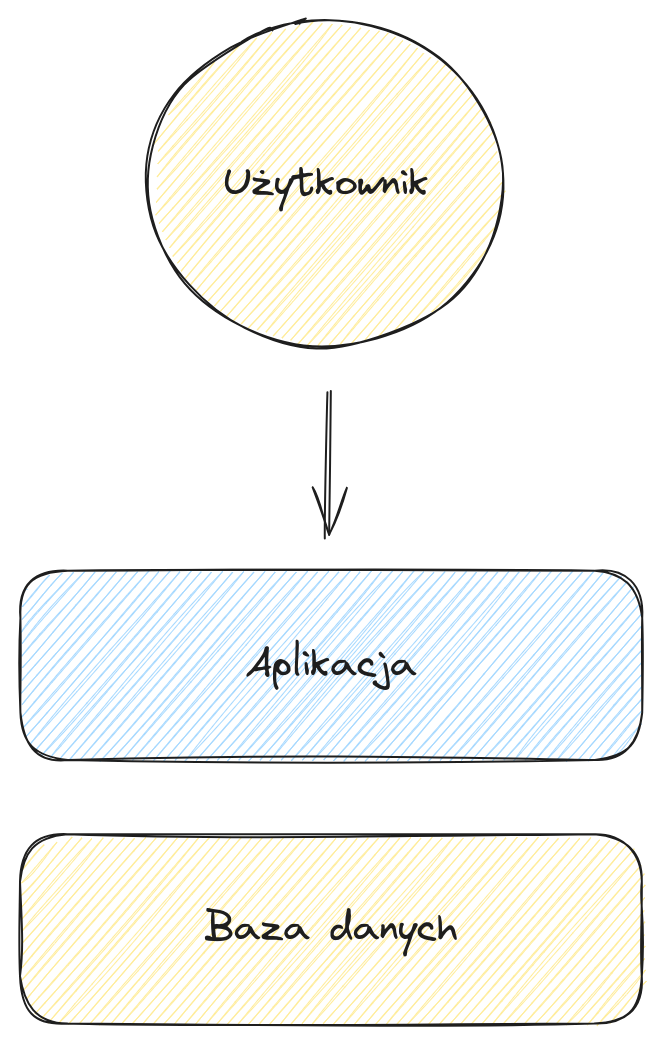
\includegraphics[width=0.5\linewidth]{rysunki/vertical_archtecture.png}
	\caption{Schemat architektury wertykalnej}
	\label{rys:veriticalArchitecture}
\end{figure}


Aby rozwiązać ten problem stosuje się architekturę horyzontalną.
Schemat architektury horyzontalnej został zaprezentowany na rysunku \ref{rys:horizontalArchitecture}.
Pośrednikiem komunikacji użytkownika z aplikacją jest urządzenie które przydziela instancję aplikacji użytkownikowi, tak, że z perspektywy użytkownika stale widoczna jest jedna aplikacja, natomiast może być uruchomionych wiele instancji w zależności od zapotrzebowania.
Kiedy ruch jest bardzo mały, tylko jedna aplikacji może być uruchomiona.
Wraz ze wzrostem obciążenia mogą być dynamicznie uruchamiane kolejne instancje aplikacji.
Jest to możliwe dzięki środowiskom chmurowym, gdzie uruchomienie kolejnej instancji aplikacji nie wymaga postawienia kolejnego urządzenia fizycznego.

\begin{figure}[!hb]
	\centering 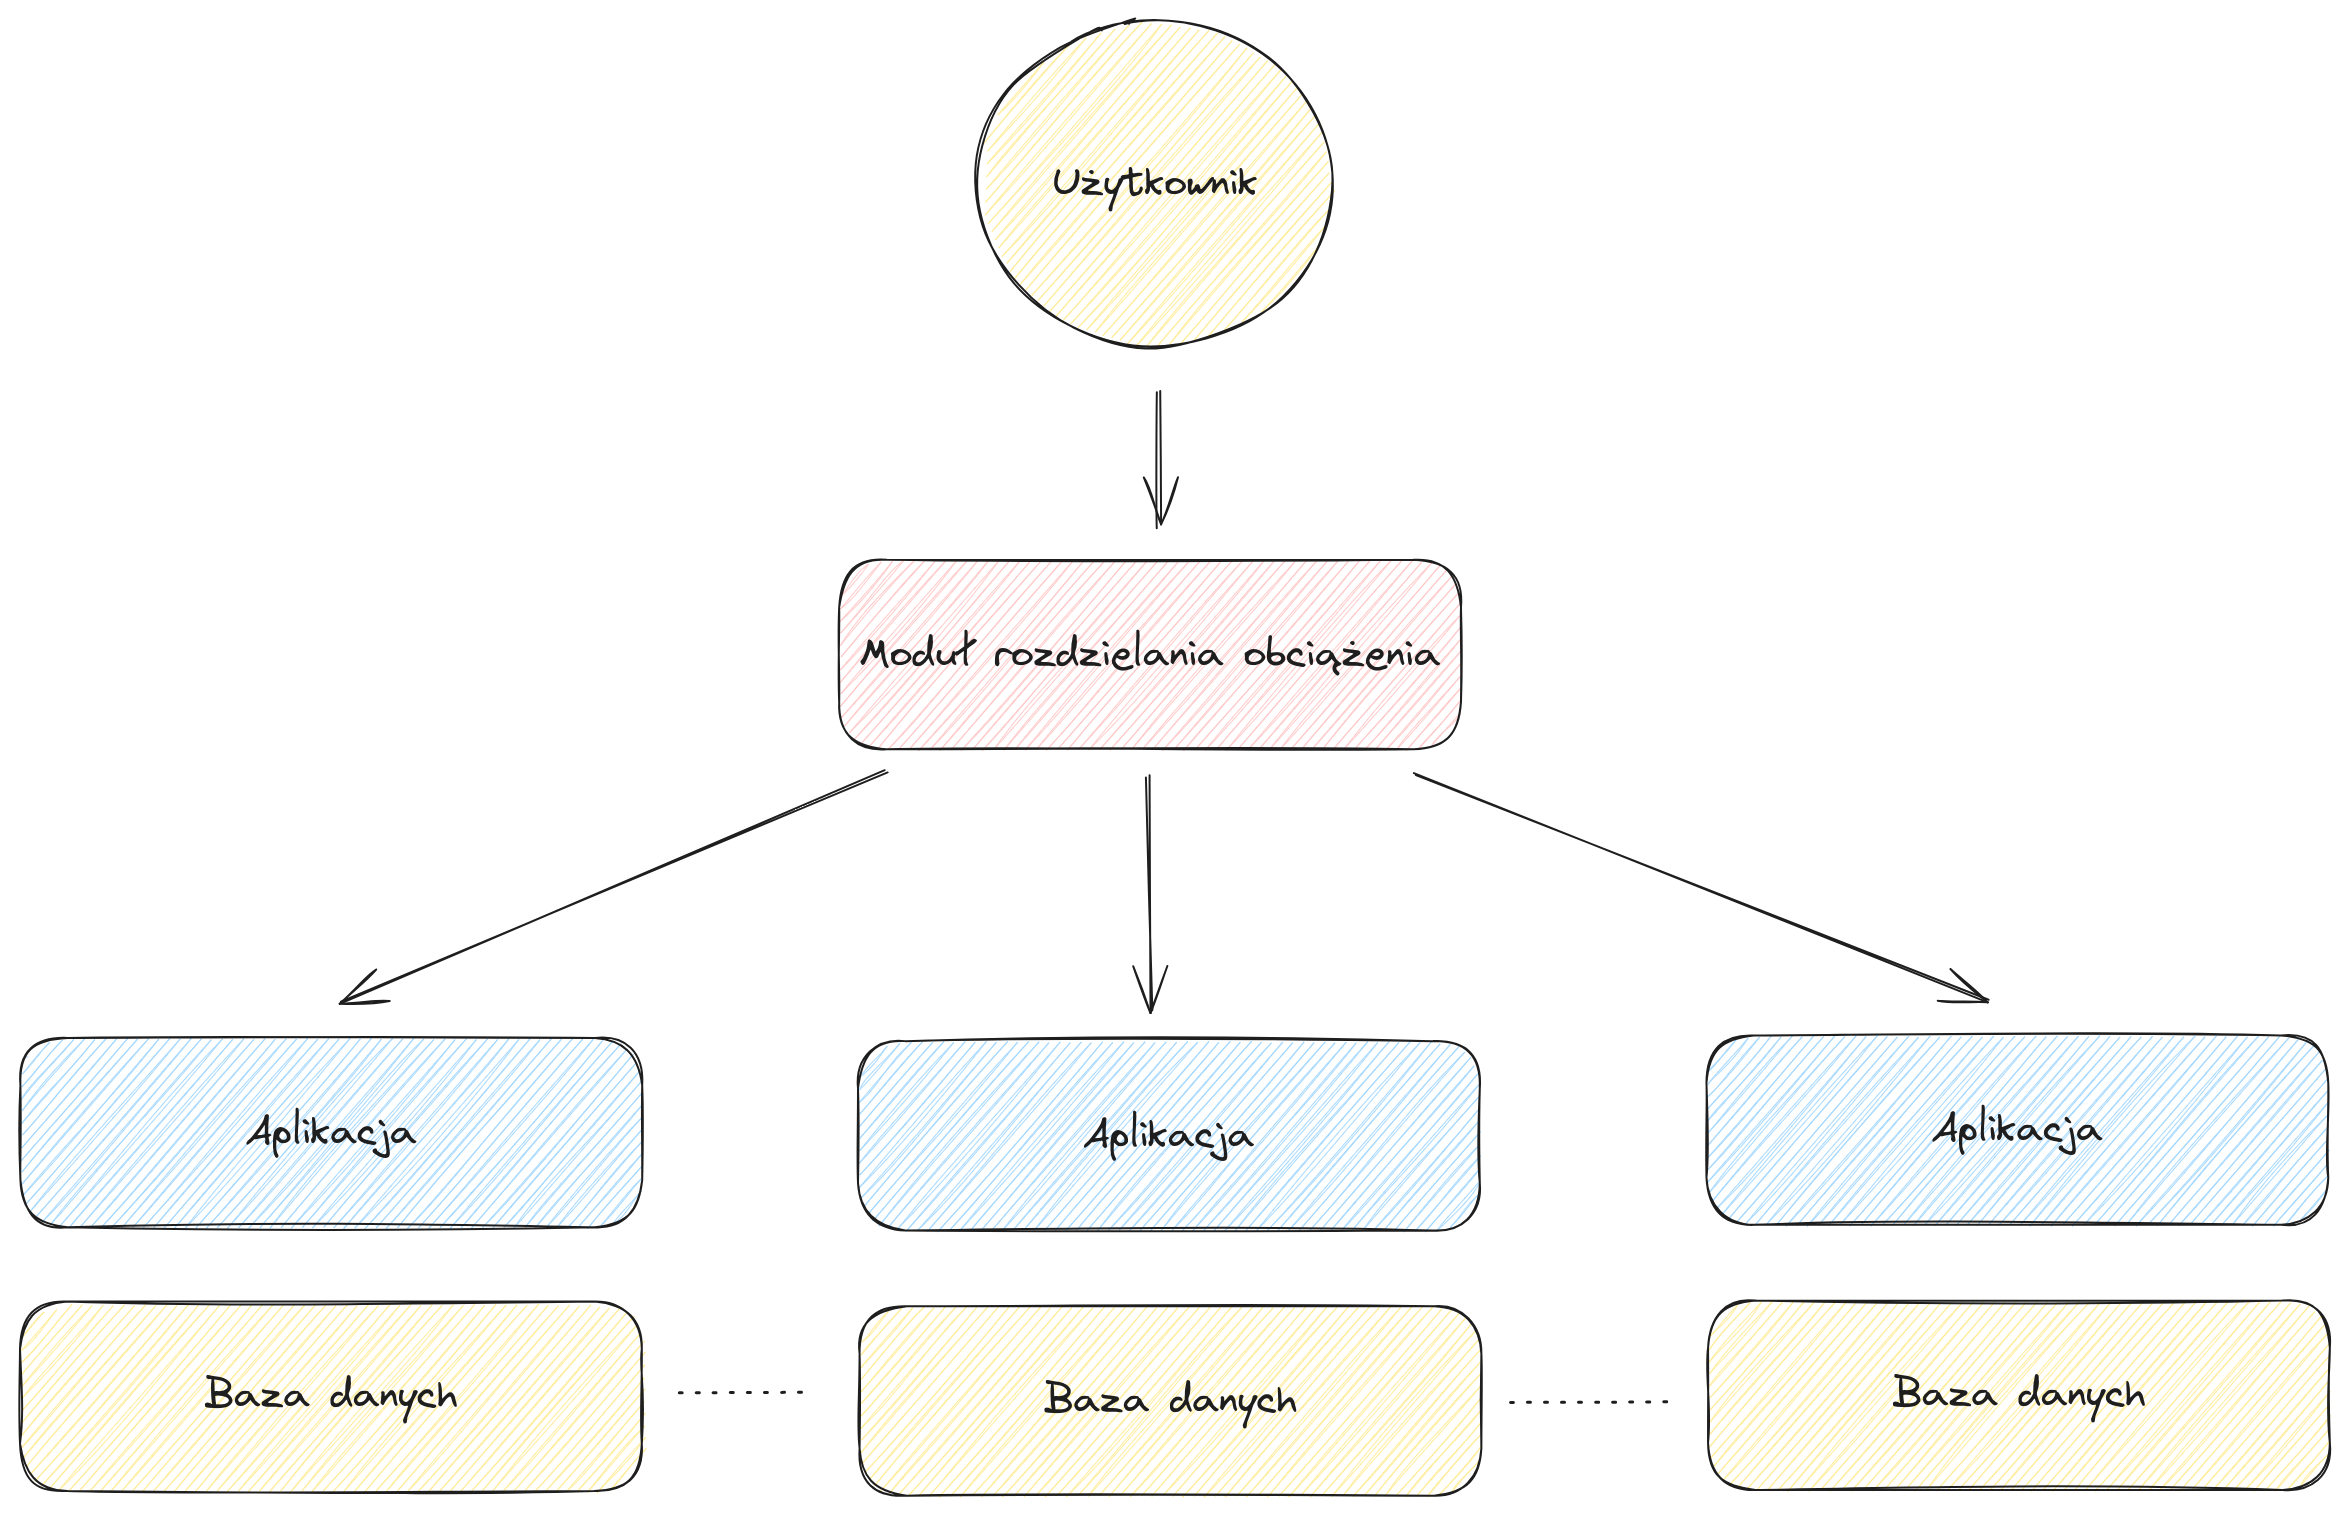
\includegraphics[width=1\linewidth]{rysunki/horizontal_archtecture.png}
	\caption{Schemat architektury horyzontalnej}
	\label{rys:horizontalArchitecture}
\end{figure}
